% To make a PDF from this source, use the pdflatex command.
\documentclass[helvetica,english,utf8,notitle,nologo]{beamer}
\usetheme{default}
\usecolortheme{seahorse}
\usepackage{graphicx}
\graphicspath{ {images/} }

\begin{document}

\title{Intro to Docker}
\author{Carlos Konstanski}

\frame{\titlepage}

\begin{frame}
  \frametitle{Presentation Materials Available Online At:}
  \href{url}{https://github.com/ckonstanski/docker-presentation}
\end{frame}

\begin{frame}
  \frametitle{Supported Platforms}

  Docker runs on Linux, Mac OSX and Windows. 

  This presentation is done entirely on Linux. From a user interface
  standpoint things should be nearly identical on Mac and Windows
  (according to the Docker website).
\end{frame}

\begin{frame}
  \frametitle{What Is Virtualization?}

  To understand containerization, it is useful to examine how it
  differs from virtualization.

  Virtualization is when an entire operating system, consisting of
  both kernel and user space, runs inside a single process within
  another operating system. The parent OS provides software-emulated
  hardware for the virtualized OS.

  The emulated hardware might be implemented entirely in software, or
  it might be a thin software wrapper around real hardware.
\end{frame}

\begin{frame}
  \frametitle{What Is a Chroot Jail?}

  Another useful concept to understand as a prerequisite to
  containerization is the chroot jail.

  Every process has access to the filesystem. By default the
  filesystem that the process sees has its root at /. A chroot jail is
  a means of limiting the process' access to the filesystem by
  restricting its / to a subdirectory.

  Every filesystem resource that the chrooted process requires must be
  present inside the chroot directory tree. It will have its own
  /usr/bin, /usr/lib, /lib, /dev, /proc, etc. with copies of all
  needed executables, shared objects, etc.

  Examples of common programs that typically run in a chroot:

  \begin{itemize}
  \item bind
  
  \end{itemize}

  Demonstration: mount a Linux filesystem from a rescue CD and chroot
  into it.
\end{frame}

\begin{frame}
  \frametitle{What Is Containerization?}

  Containerization is something in between a chroot and a virtual
  machine, more closely resembling a chroot.

  There is no kernel space in a container, only userspace. Since the
  parent OS is providing the kernel space, there is no need for
  hardware emulation.

  The linux features that make containers possible are namespaces and
  cgroups.

  A quick read to familiarize yourself with the basics of namespaces
  and cgroups:

  https://jvns.ca/blog/2016/10/10/what-even-is-a-container/

  There are also some extra goodies that docker supplies which we will
  look at soon.
\end{frame}

\begin{frame}
  \frametitle{What Is Docker?}

  Docker is a system that uses namespaces and cgroups at its core,
  plus some extra goodies on top, to provide a very easy to use
  containerization platform. Some of these goodies are:

  \begin{itemize}
  \item A registry where prebuilt containers can be stored
  \item A simple means to build containers with customizations
  \item Private networking for free
  \item A means to mount directories on the host filesystem
  \end{itemize}

  Other such platforms exist, for instance LXC. Docker is just the
  most popular.
\end{frame}

\begin{frame}
  \frametitle{Docker Registry}

  The Docker Registry is a storage and retrieval system for prebuilt
  Docker containers. You can either use the public registry, or you
  can set up your own private one. The public registry is called
  Docker Hub.
\end{frame}

\begin{frame}
  \frametitle{Using Docker: Docker Hub}

  Docker Hub is a public web service: https://hub.docker.com/explore/

  It contains lots of free prebuilt docker images. An image can be
  downloaded by using the docker pull command or by referenceing it in
  your Dockerfile (more on this later).
\end{frame}

\begin{frame}
  \frametitle{Docker Pull}

  Example: using the docker pull command to download the latest Ubuntu
  LTS image.

  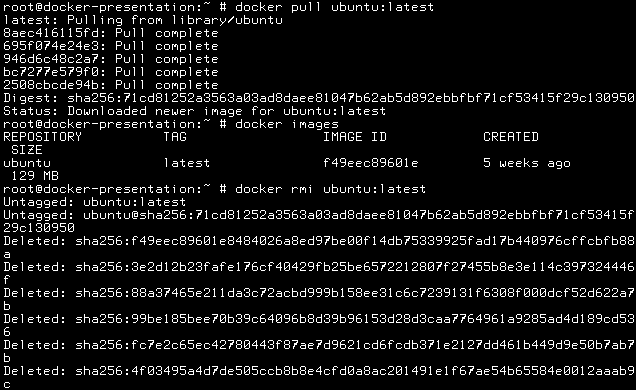
\includegraphics[scale=0.48]{image_1}
\end{frame}

\begin{frame}
  \frametitle{Dockerfile}

  

  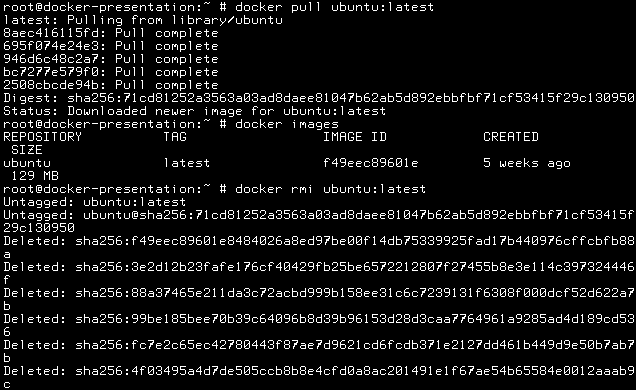
\includegraphics[scale=0.48]{image_1}
\end{frame}





% \begin{frame}
%   \frametitle{Ruby Syntax: while-loop}

%   A while-loop with conditional at end:

%   \includegraphics[scale=0.53]{src_1}

%   \includegraphics[scale=0.5]{out_1}

%   A while-loop with conditional at beginning:

%   \includegraphics[scale=0.53]{src_2}

%   \includegraphics[scale=0.5]{out_2}
% \end{frame}





\end{document}
